%\documentclass[11pt,letterpaper]{article}
\documentclass[14pt,letterpaper]{extarticle}

% ----------------------------------
%            PAQUETES
% ----------------------------------
\usepackage[spanish]{babel}
\usepackage[utf8]{inputenc}
\usepackage[T1]{fontenc}
\usepackage{lmodern}  
\usepackage{csquotes}
\usepackage{setspace}           % Interlineado
\usepackage{geometry}           % Márgenes

							          % Hipervínculos
\usepackage{titlesec}           % Formato de títulos
\usepackage{tocloft}            % Formato de tabla de contenido
\usepackage{filecontents}
\usepackage{graphicx}
\usepackage{apacite}            % Estilo APA
\usepackage{indentfirst}        % Sangría en primer párrafo


\onehalfspacing                 % Interlineado 1.5
\graphicspath{{./Imagenes/}}




% ----------------------------------
%            FORMATO APA
% ----------------------------------
\geometry{left=2.54cm, right=2.54cm, top=2.54cm, bottom=2.54cm}
\onehalfspacing     % Interlineado 1.5

% Estilo de títulos APA
\titleformat{\section}{\normalfont\bfseries\large}{\thesection.}{0.5em}{}
\titleformat{\subsection}{\normalfont\bfseries\normalsize}{\thesubsection.}{0.5em}{}

% ----------------------------------
%        PORTADA TIPO APA
% ----------------------------------
\title{\textbf{Título del Informe}}
\author{Marlon Iván Carreto Rivera}
\date{\today}


\usepackage{pdfpages}
\usepackage{hyperref} 
\hypersetup{
	colorlinks=true,
	linkcolor=black,
	urlcolor=black,
	citecolor=black
}









% ----------------------------------
\begin{document}
	
		
\includepdf[pages=-,pagecommand={}]{Caratula/Caratulaanteproyecto.pdf}
	%%
\includepdf{Caratula/Caratulaanteproyecto.pdf}
	%\maketitle
	\thispagestyle{empty}


	\newpage
	
	
	
	
	
	
	% ----------------------------------
	%      TABLA DE CONTENIDO
	% ----------------------------------
	\renewcommand{\contentsname}{Contenido}
	\tableofcontents
	\newpage
	

	
	% ----------------------------------
	%        CONTENIDO DEL INFORME
	% ----------------------------------
	
	%%%\section*{Introducción }
	
	% --- Introducción (sin numerar, con link funcional) ---
	%\phantomsection
	\section*{Introducción}
	%\addcontentsline{toc}{section}{Introducción}
	
		
	\addcontentsline{toc}{section}{Introducción}
	El presente anteproyecto consiste en el desarrollo del diseño preliminar de un edificio destinado a servicios de salud, denominado Hospital Luz Vida, el cual se proyecta construir en el municipio de San Juan Ostuncalco, departamento de Quetzaltenango, Guatemala. Este proyecto se realiza como parte del curso de Maestría en Tipología Estructural y tiene como finalidad aplicar los conocimientos adquiridos sobre el diseño y concepción estructural de edificaciones, integrando criterios técnicos, funcionales y normativos que permitan plantear una propuesta viable y acorde al contexto del país.
	
	 Debido a la naturaleza del uso del edificio, es fundamental considerar aspectos como la seguridad estructural, la estabilidad, la adecuada transmisión de cargas y el comportamiento de la estructura ante acciones externas, especialmente aquellas relacionadas con la actividad sísmica característica del territorio guatemalteco.
	
	En este sentido, el desarrollo del anteproyecto contempla la aplicación de criterios establecidos en normas y reglamentos reconocidos para el diseño estructural. Entre ellos destacan las disposiciones del ACI (American Concrete Institute) para el diseño de estructuras de concreto reforzado, así como las Normas de Seguridad Estructural de Guatemala (NSE), las cuales establecen los lineamientos mínimos para garantizar el desempeño adecuado de las edificaciones frente a cargas gravitacionales, sísmicas y otras acciones que puedan afectar su integridad. La correcta aplicación de estas normas permite plantear soluciones estructurales que contribuyan a la seguridad de los usuarios y a la durabilidad de la edificación.
	
	Asimismo, el anteproyecto busca integrar de manera coherente la distribución arquitectónica del hospital con el sistema estructural propuesto, procurando que la disposición de columnas, vigas y elementos estructurales facilite la funcionalidad de los espacios y permita una adecuada organización de las áreas médicas, administrativas y de servicios. 
	

	
	\section*{Objetivos}
		
	\addcontentsline{toc}{section}{Objetivos}
	\subsection*{Objetivo General}
	Desarrollar el anteproyecto estructural y arquitectónico del Hospital Luz Vida, un edificio hospitalario de cinco niveles ubicado en el municipio de San Juan Ostuncalco, Quetzaltenango, aplicando criterios de diseño estructural, funcionalidad espacial y normativas vigentes como el ACI y las Normas de Seguridad Estructural de Guatemala (NSE), con el fin de proponer una edificación segura, funcional y acorde a las necesidades del contexto.
	
	\subsection*{Objetivo Específico}
	\begin{enumerate}
		\item Definir la configuración arquitectónica del edificio, estableciendo la distribución de los espacios hospitalarios en cada nivel de acuerdo con criterios de funcionalidad, circulación y uso adecuado de las áreas médicas y administrativas.
		\item Proponer un sistema estructural adecuado para la edificación, considerando las dimensiones del proyecto, la altura del edificio y las condiciones sísmicas del territorio guatemalteco.
		\item Aplicar criterios de diseño estructural basados en normas técnicas, especialmente las disposiciones del ACI para concreto reforzado y las Normas de Seguridad Estructural de Guatemala (NSE), con el propósito de garantizar la estabilidad y seguridad del edificio.
		\item Elaborar los planos básicos del anteproyecto, incluyendo plantas de los niveles y elevaciones debidamente acotadas, que permitan representar de forma clara la propuesta arquitectónica y estructural del Hospital Luz Vida.
	\end{enumerate}
	
	% ----------------------------------
	\section{Descripción el Proyecto}
	El proyecto consiste en el planteamiento y desarrollo del anteproyecto arquitectónico y estructural de una edificación hospitalaria denominada Hospital Luz Vida, la cual estará destinada a brindar servicios de atención médica a la población del municipio de San Juan Ostuncalco, en el departamento de Quetzaltenango, Guatemala. La propuesta busca establecer una solución conceptual que permita organizar de manera adecuada los diferentes espacios requeridos en una infraestructura de salud, tomando en cuenta aspectos funcionales, estructurales y normativos.

	
	La edificación se proyecta con una altura de cinco niveles y una configuración en planta de aproximadamente 25 metros por 30 metros. Estas dimensiones permiten desarrollar áreas suficientes para la distribución de los distintos ambientes hospitalarios, tales como áreas de atención médica, servicios administrativos, circulación de pacientes, así como espacios destinados al apoyo operativo del hospital. La organización de los niveles busca optimizar el funcionamiento interno del edificio y facilitar el acceso y desplazamiento de usuarios, personal médico y pacientes
	\newpage
	
	\subsection{Cantidad de Niveles}
	El proyecto del Hospital Luz Vida contempla el diseño de una edificación de cinco niveles, los cuales han sido planteados con el propósito de distribuir de manera adecuada las diferentes áreas necesarias para el funcionamiento de un centro de atención médica. La altura del edificio permite organizar los espacios hospitalarios de forma eficiente, separando las áreas de atención al público, servicios médicos especializados, áreas administrativas y zonas de apoyo.
	
	En cuanto a la altura de los niveles, el primer nivel contará con una altura de 3.50 metros, con el objetivo de proporcionar mayor amplitud en las áreas de acceso principal, recepción y servicios de atención al público. Por su parte, los niveles superiores (del segundo al quinto nivel) tendrán una altura de 3.00 metros cada uno, dimensiones que permiten mantener condiciones adecuadas de ventilación, iluminación y funcionamiento de las diferentes áreas hospitalarias.
	\newpage
	
	
	\subsection{Área por Nivel}
	El edificio propuesto para el Hospital Luz Vida presenta una configuración rectangular en planta, con dimensiones de 25 metros en sentido norte–sur y 30 metros en sentido oriente–poniente. Estas dimensiones permiten desarrollar una superficie adecuada para la distribución de los distintos espacios hospitalarios dentro de cada nivel.
	
	A partir de estas dimensiones, el área bruta por nivel del edificio es de 750 m², lo que equivale aproximadamente a 8,072 ft². Esta superficie constituye el área total disponible para la organización de las diferentes áreas funcionales del hospital.
	
	Asimismo, el diseño contempla un espacio lateral destinado a ventilación e iluminación natural, ubicado en uno de los costados del edificio. Este espacio tiene dimensiones aproximadas de 3 metros por 4 metros, lo que representa un área de 12 m² (aproximadamente 129 ft²). La incorporación de esta abertura permite mejorar las condiciones de ventilación y el ingreso de luz natural hacia el interior de la edificación, contribuyendo a generar ambientes más confortables para los usuarios y el personal del hospital.
	
	Considerando este espacio destinado a ventilación, el área neta aproximada por nivel del edificio es de 738 m², equivalente a aproximadamente 7,943 ft², superficie que será utilizada para la distribución de los diferentes ambientes hospitalarios.
	
	\subsection{Materiales y Acabados de la Edificación}
	La selección de materiales y acabados para el Hospital Luz Vida se plantea considerando criterios de durabilidad, higiene, facilidad de mantenimiento y seguridad para los usuarios. Debido a la naturaleza de las actividades que se desarrollan en un centro hospitalario, los materiales deben cumplir con características específicas que permitan mantener condiciones adecuadas de limpieza, resistencia al desgaste y confort para pacientes y personal médico.
	
		\subsection{Piso}
		Para las áreas interiores del edificio se propone la utilización de pisos vinílicos hospitalarios, con dimensiones aproximadas de 60 cm x 60 cm, fabricados principalmente a base de cloruro de polivinilo (PVC). Este tipo de revestimiento es ampliamente utilizado en edificaciones destinadas a servicios de salud debido a sus propiedades de resistencia, durabilidad y facilidad de mantenimiento.
		
		\begin{figure}[h]
			\centering
			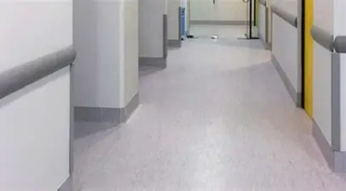
\includegraphics[width=0.8\textwidth]{piso}
			
		\end{figure}
		
		Los pisos vinílicos se caracterizan por ofrecer una superficie continua, impermeable y de fácil limpieza, lo cual resulta fundamental en ambientes hospitalarios donde se requiere mantener altos estándares de higiene y control sanitario. Asimismo, este material presenta una buena resistencia al desgaste producido por el tránsito constante de personas, camillas y equipo médico.
		
		Otra ventaja importante de este tipo de piso es su flexibilidad y capacidad de absorción de impactos, lo cual contribuye a mejorar el confort durante la circulación dentro del edificio y reduce el nivel de ruido generado por el tránsito. Además, su instalación permite generar superficies antideslizantes, lo que incrementa la seguridad para pacientes, visitantes y personal médico.
		
		
		
		\begin{figure}[h]
			\centering
			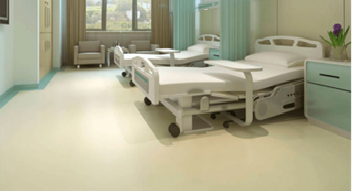
\includegraphics[width=0.8\textwidth]{piso2}
			
		\end{figure}
		
		\subsection{Cielo Falso}
		
		El edificio contará con la instalación de cielos falsos o plafones suspendidos, los cuales cumplirán una función tanto estética como funcional dentro de los diferentes ambientes hospitalarios. Estos sistemas permiten ocultar instalaciones eléctricas, redes de climatización, sistemas de iluminación y otros elementos técnicos necesarios para el funcionamiento del hospital.
		
		\begin{figure}[h]
			\centering
			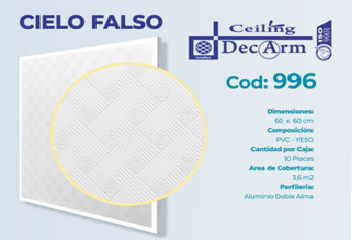
\includegraphics[width=0.8\textwidth]{cielo1}
			
		\end{figure}
		
		Para la instalación de los cielos falsos se empleará una estructura metálica suspendida, debidamente anclada a la losa estructural superior mediante sistemas de fijación adecuados que garanticen estabilidad y seguridad. Sobre esta estructura se colocarán paneles modulares que faciliten el acceso a las instalaciones cuando sea necesario realizar mantenimiento o reparaciones.
		
			\begin{figure}[h]
			\centering
			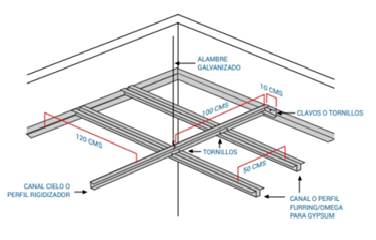
\includegraphics[width=0.8\textwidth]{cielo2}
			
		\end{figure}
		
		En edificaciones hospitalarias es importante que los materiales utilizados en los cielos falsos presenten características como resistencia a la humedad, fácil limpieza y propiedades acústicas, ya que estas contribuyen a mejorar las condiciones de confort en las diferentes áreas del hospital. Además, la correcta instalación del cielo falso permite integrar adecuadamente los sistemas de iluminación artificial y ventilación, favoreciendo un ambiente interior más adecuado para el desarrollo de las actividades médicas.
		
		
		
		
	
	\subsection{Uso de la Edificación}
	Contenido aquí…
	
	\subsection{Ubicación donde se Construirá}
	Contenido aquí…
	
	
	
	
	\section{Planos del Proyecto}
	
	\subsection{Planos de planta de los niveles típicos, con cotas }
	Contenido aquí…
	
	\subsection{Elevaciones con Cotas}
	Contenido aquí…
	
	% ----------------------------------
	%%\section{Marco Normativo}
	
	\section{Normativa Aplicada}
	
	El anteproyecto estructural del edificio hospitalario de cinco niveles, con dimensiones en planta de $25\,m \times 30\,m$, se desarrolla con base en la normativa estructural vigente en Guatemala y en normas internacionales aplicables al diseño de estructuras de concreto reforzado. Estas normas establecen los criterios para garantizar la seguridad estructural frente a cargas gravitacionales, cargas sísmicas y otras acciones que puedan afectar la edificación.
	
	\subsection{Normativa Nacional}
	
	El diseño estructural se fundamenta principalmente en las Normas de Seguridad Estructural (NSE) emitidas por la \textbf{Asociación Guatemalteca de Ingeniería Estructural y Sísmica (AGIES)}. Estas normas establecen los requisitos mínimos para el diseño y construcción segura de edificaciones en el territorio nacional.
	
	\subsubsection{NSE 1 -- Generalidades}
	
	La norma NSE 1 establece los principios generales para la aplicación de las normas estructurales y define las responsabilidades de los profesionales involucrados en el diseño y supervisión estructural. En el presente proyecto se consideran principalmente los siguientes apartados:
	
	\begin{itemize}
		\item Sección 1.3: Alcance de las normas.
		\item Sección 1.4: Responsabilidad del diseñador estructural.
		\item Sección 1.5: Supervisión técnica estructural.
	\end{itemize}
	
	\subsubsection{NSE 2 -- Demandas estructurales y condiciones del sitio}
	
	Esta norma establece las cargas que deben considerarse en el diseño estructural, así como los parámetros relacionados con acciones sísmicas y cargas de viento. Los apartados utilizados en el presente anteproyecto incluyen:
	
	\begin{itemize}
		\item Capítulo 2: Cargas muertas.
		\item Capítulo 3: Cargas vivas.
		\item Capítulo 4: Aspectos sísmicos.
		\item Capítulo 5: Acciones de viento.
	\end{itemize}
	
	De acuerdo con esta normativa, los hospitales se clasifican como \textbf{estructuras esenciales}, por lo que deben diseñarse con un mayor nivel de protección sísmica y un factor de importancia mayor que el utilizado en edificaciones convencionales.
	
	\subsubsection{NSE 2.1 -- Estudios geotécnicos}
	
	La norma NSE 2.1 establece los requisitos para la investigación del suelo y la determinación de parámetros geotécnicos necesarios para el diseño de cimentaciones. En el presente proyecto se consideran los siguientes aspectos:
	
	\begin{itemize}
		\item Investigaciones geotécnicas del sitio.
		\item Clasificación del suelo.
		\item Determinación de parámetros geotécnicos de diseño.
	\end{itemize}
	
	\subsubsection{NSE 3 -- Diseño estructural de edificaciones}
	
	Esta norma regula el análisis estructural y los criterios para el diseño sísmico de edificaciones. Los aspectos considerados en el presente anteproyecto incluyen:
	
	\begin{itemize}
		\item Sistemas estructurales aplicables a edificaciones.
		\item Métodos de análisis estructural.
		\item Determinación de fuerzas sísmicas de diseño.
		\item Control de derivas y desplazamientos laterales.
	\end{itemize}
	
	El periodo fundamental aproximado de la estructura puede estimarse mediante la expresión establecida en esta norma:
	
	\[
	T_a = K_t (h_n)^x
	\]
	
	donde $h_n$ representa la altura total de la estructura, mientras que $K_t$ y $x$ dependen del sistema estructural utilizado.
	
	\subsection{Normativa Internacional}
	
	Para el diseño de los elementos estructurales de concreto reforzado se utiliza el código del \textbf{American Concrete Institute (ACI)}.
	
	\subsubsection{ACI 318-19}
	
	El código ACI 318-19 establece los requisitos para el diseño, análisis y detallado de estructuras de concreto reforzado. En el desarrollo del presente anteproyecto se consideran principalmente los siguientes capítulos:
	
	\begin{itemize}
		\item Capítulo 1: Generalidades.
		\item Capítulo 5: Cargas y combinaciones.
		\item Capítulo 9: Factores de reducción de resistencia.
		\item Capítulo 18: Requisitos sísmicos para estructuras de concreto.
		\item Capítulo 22: Resistencia de secciones.
		\item Capítulo 23: Diseño a cortante y torsión.
		\item Capítulo 24: Requisitos de servicio y deflexiones.
		\item Capítulo 25: Detallado del refuerzo.
		\item Capítulo 26: Requisitos constructivos.
	\end{itemize}
	
	\subsection{Normas complementarias}
	
	Adicionalmente, para la determinación de cargas y la clasificación de edificaciones se consideran normas internacionales complementarias:
	
	\begin{itemize}
		\item ASCE 7: Minimum Design Loads for Buildings and Other Structures.
		\item International Building Code (IBC): Clasificación de ocupaciones y criterios generales de seguridad estructural.
	\end{itemize}
	
	Estas normas permiten establecer criterios adicionales para el cálculo de cargas, la determinación de factores de importancia y la clasificación de edificaciones destinadas a servicios esenciales, como es el caso de hospitales.
	
	
	
	
	
	
	
	
	
	
	
	
	
	
	
	
	
	
	
	%%%%%%%%%%%%%%%%%%%%%%%%%%%%%%%%%%%%%%%%%%%%%%%%555
	
		\newpage
	
	% ----------------------------------
	\section*{Conclusiones}
	\addcontentsline{toc}{section}{Conclusiones}
	El desarrollo del anteproyecto del Hospital Luz Vida permitió establecer una propuesta arquitectónica y estructural coherente con las necesidades funcionales de una edificación destinada a la prestación de servicios de salud, tomando como base las condiciones propias del municipio de San Juan Ostuncalco y del contexto sísmico de Guatemala. A través del análisis de los requerimientos espaciales y operativos del edificio, fue posible definir una distribución arquitectónica adecuada para los cinco niveles proyectados, asegurando la correcta organización de las áreas médicas, administrativas y de apoyo, así como una circulación eficiente para usuarios y personal.
	
	Asimismo, la propuesta estructural se fundamentó en la aplicación de criterios y normativas reconocidas, especialmente las disposiciones del ACI para estructuras de concreto reforzado y las Normas de Seguridad Estructural de Guatemala (NSE). El uso de estas guías permitió garantizar que el planteamiento estructural responda apropiadamente a las demandas gravitacionales y sísmicas que caracterizan al territorio nacional, aportando estabilidad, seguridad y durabilidad a la edificación.
	

	
	% ----------------------------------
	%         BIBLIOGRAFÍA APA
	% ----------------------------------
	\newpage
	\bibliographystyle{apacite}
	\renewcommand{\refname}{Referencias}
	
	\bibliography{bibliografia}
	
	
	\renewcommand{\refname}{Referencias}
	
		 American Concrete Institute. (2019). \textit{Building code requirements for structural concrete (ACI 318-19) and commentary}. American Concrete Institute.
		
	
		 American Concrete Institute. (2014). \textit{Guide to durable concrete (ACI 201.2R-16)}. American Concrete Institute.
	

		
	
		
		American Concrete Institute. (2014). \textit{Guide to durable concrete (ACI 201.2R-16)}. American Concrete Institute.
		
		Asociación Guatemalteca de Ingeniería Estructural y Sísmica. (2018). \textit{Norma de seguridad estructural NSE 1: Cargas para diseño estructural}. AGIES.
		
		 Asociación Guatemalteca de Ingeniería Estructural y Sísmica. (2018). \textit{Norma de seguridad estructural NSE 2: Diseño por sismo}. AGIES.
		
		 Asociación Guatemalteca de Ingeniería Estructural y Sísmica. (2018). \textit{Norma de seguridad estructural NSE 3: Concreto estructural}. AGIES.
		
		 Asociación Guatemalteca de Ingeniería Estructural y Sísmica. (2018). \textit{Norma de seguridad estructural NSE 4: Acero estructural}. AGIES.
		
		 Asociación Guatemalteca de Ingeniería Estructural y Sísmica. (2018). \textit{Norma de seguridad estructural NSE 5: Cimentaciones}. AGIES.
		
		 Asociación Guatemalteca de Ingeniería Estructural y Sísmica. (2018). \textit{Normas de seguridad estructural de edificaciones en Guatemala}. AGIES.
		
		Ching, F. D. K. (2015). \textit{Building construction illustrated} (5th ed.). John Wiley \& Sons.
		
	
	
	
\end{document}